\section{Unfolding}
%%%%%%%%%%%%%%%%%%%%%%%%%%%%%%%%%%%%%%%%%%%%%%%%%%%%%%%%%%%%%%%%%%%%%%
\label{sec:Unfolding}

To facilitate comparisons with theoretical predictions or other experimental results, the signal
extracted performing the fit has to be corrected for detector resolution and
efficiency effects and for the efficiency of the selection defined in the
analysis.
An unfolding procedure is used relying on the \textsc{RooUnfold} package
\cite{Adye:2011gm}, which provides the tools to run various unfolding
algorithms.

The basic principle behind the unfolding procedure in this analysis is to use MC signal samples
to make the ``true'' distribution of the variable of interest, which is obtained using simulated events before particle interaction with the detector, and the same distribution obtained using events reconstructed after the full \textsc{Geant4} simulation of the CMS detector
and event reconstruction. 

These two distributions are used to calculate the detector response matrix $M$:
\begin{equation}\label{eq:resp_matrix}
R_{i}^{\rm {MC}} = \sum_{j=1}^{n} M_{ij}T_{j}^{\rm {MC}} \quad ,
\end{equation}

\noindent where $T^{\rm{MC}}$ and $R^{\rm{MC}}$ are two $n$-dimensional vectors
representing the distribution before and after event processing through CMS
simulation and reconstruction. The dimension $n$ of the two vectors corresponds 
to the number of bins in the distributions, equal to six in this analysis.
The response matrix $M$ includes all the effects related to the detector and analysis selection that affect the $R^{\rm{MC}}$ distribution.
The goal of the unfolding procedure is to obtain the $T^{\rm{truth}}$ distribution starting from the measured
$R^{\rm{observed}}$ distribution by inverting the matrix $M$.
%To avoid the large variance and strong negative correlation between the neighbouring bins~\cite{Cowan:2002in}, 

Given the finite data statistical accuracy, a simple inversion could lead to large fluctuations between bins in the unfolded result. In particular, if the off-diagonal elements of the response matrix are sizeable, the unfolded distribution has large variance and strong negative correlations between the neighbouring bins~\cite{Cowan:2002in}. Several unfolding methods with regularization are available in literature, such as a method based on the Bayes' theorem, which overcomes the unfolding instability using an iterative procedure~\cite{DAgostini:1994zf}.

The unfolding procedure in this analysis relies on the Singular Value Decomposition (SVD)~\cite{Hocker:1995kb} method based on the Tikhonov regularization function. Such method introduces a regularization function that controls the smoothness of the distribution and depends generally on one regularization parameter, which can be controlled to achieve the desired degree of smoothness.
The choice of the regularization parameter is particularly critical, and it should represent an optimal trade-off between taming the fluctuations in the unfolded result, and biasing the unfolded distribution.
The main feature of this method is the use of the singular value decomposition of the response matrix, including an additional term to suppress the oscillatory component of the solution, i.e. the regularization term, which represents some \textit{a priori} knowledge of the final solution.
The regularization parameter $k_\mathrm{reg}$ is chosen to obtain results that are robust against numerical instabilities and statistical fluctuations, following the prescription described in Ref.~\cite{Hocker:1995kb}. This prescription consists in the diagonalization of the response matrix using the SVD approach and in the subsequent calculation of the vector $\vec{d}$, whose values $d_i$ represent the measured distribution expressed in a specific base defined by the SVD decomposition. Plotting $\log|d_i|$ as a function of $i$, where $i$ is related to the amount of regularization, one should obtain a curve that flattens out at some value of $i$. The regularization parameter corresponding to that value represents the optimal $k_\mathrm{reg}$ choice. The parameter obtained using this prescription is $k_\mathrm{reg} = 3$.

The detector response matrix is built as a two-dimensional histogram, with the generator-level \pth{} on the $y$ axis and the same variable after the reconstruction on the $x$ axis, using the same binning for both distributions.

The resulting matrix, including all signal sources and normalized by row, is shown in Fig.~\ref{fig:matrix}(a).
The diagonal bins correspond to the purity $P$, defined in Eq.\eqref{eq:purity}. The same matrix, normalized by column, is shown in Fig.~\ref{fig:matrix}(b). In this case the diagonal bins correspond to the stability $S$, defined as the ratio of the number of events generated and reconstructed in a given bin, and the number of events reconstructed in that bin. The $S$ and $P$ parameters provide an estimate of the \pth resolution and migration effects, the main source being the limited resolution in the measurement of \MET.

\begin{figure}[htb]
\centering
\subfigure[Response matrix normalized by row]{
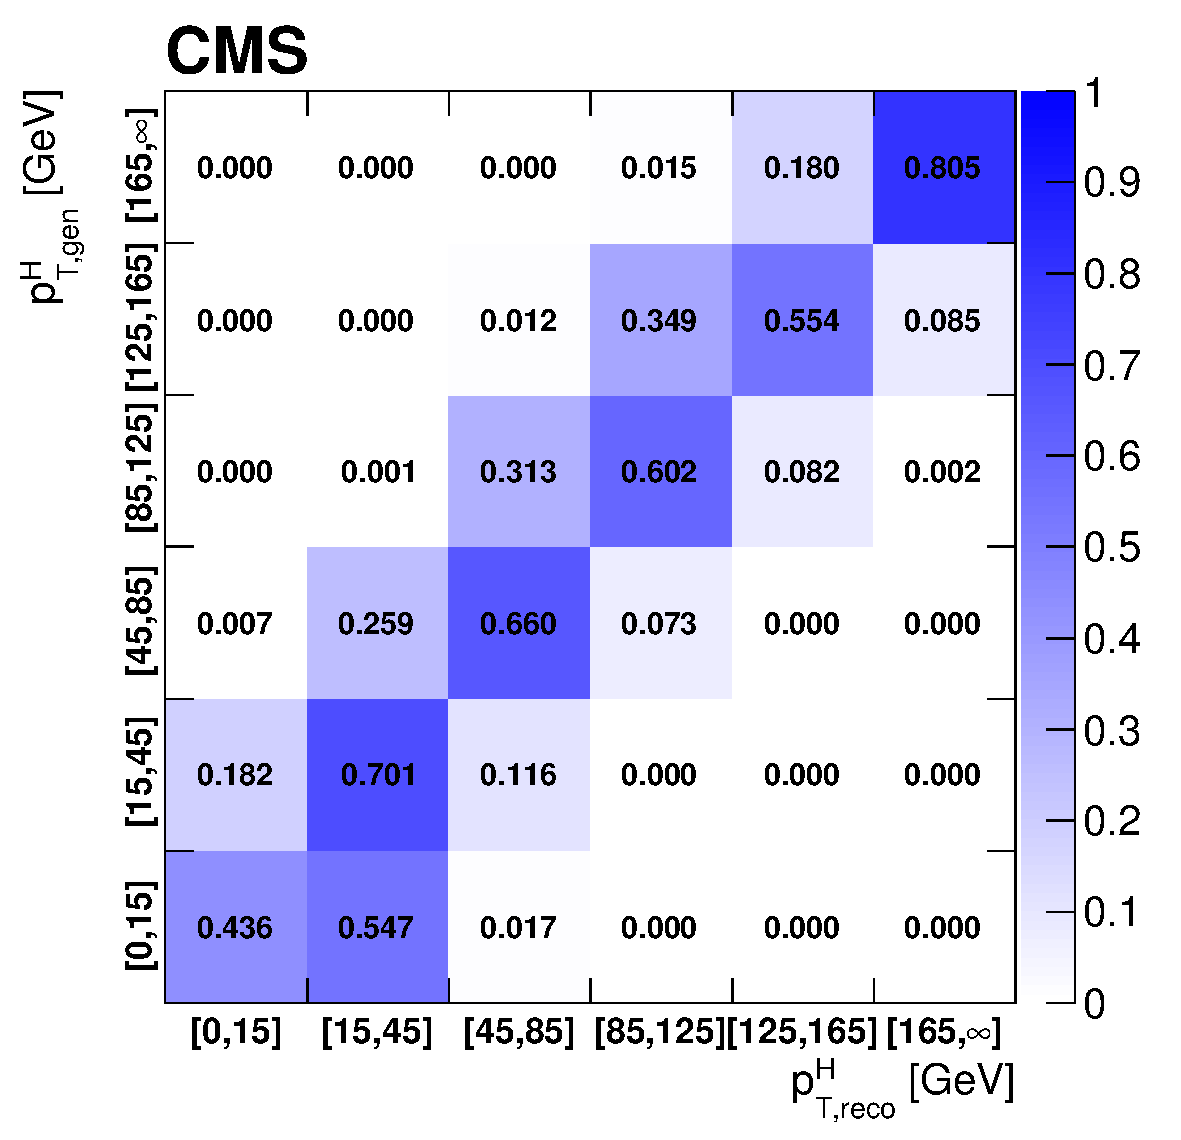
\includegraphics[width=0.45\textwidth]{images/matrix_byrow_paper.pdf}
}
\subfigure[Response matrix normalized by column]{
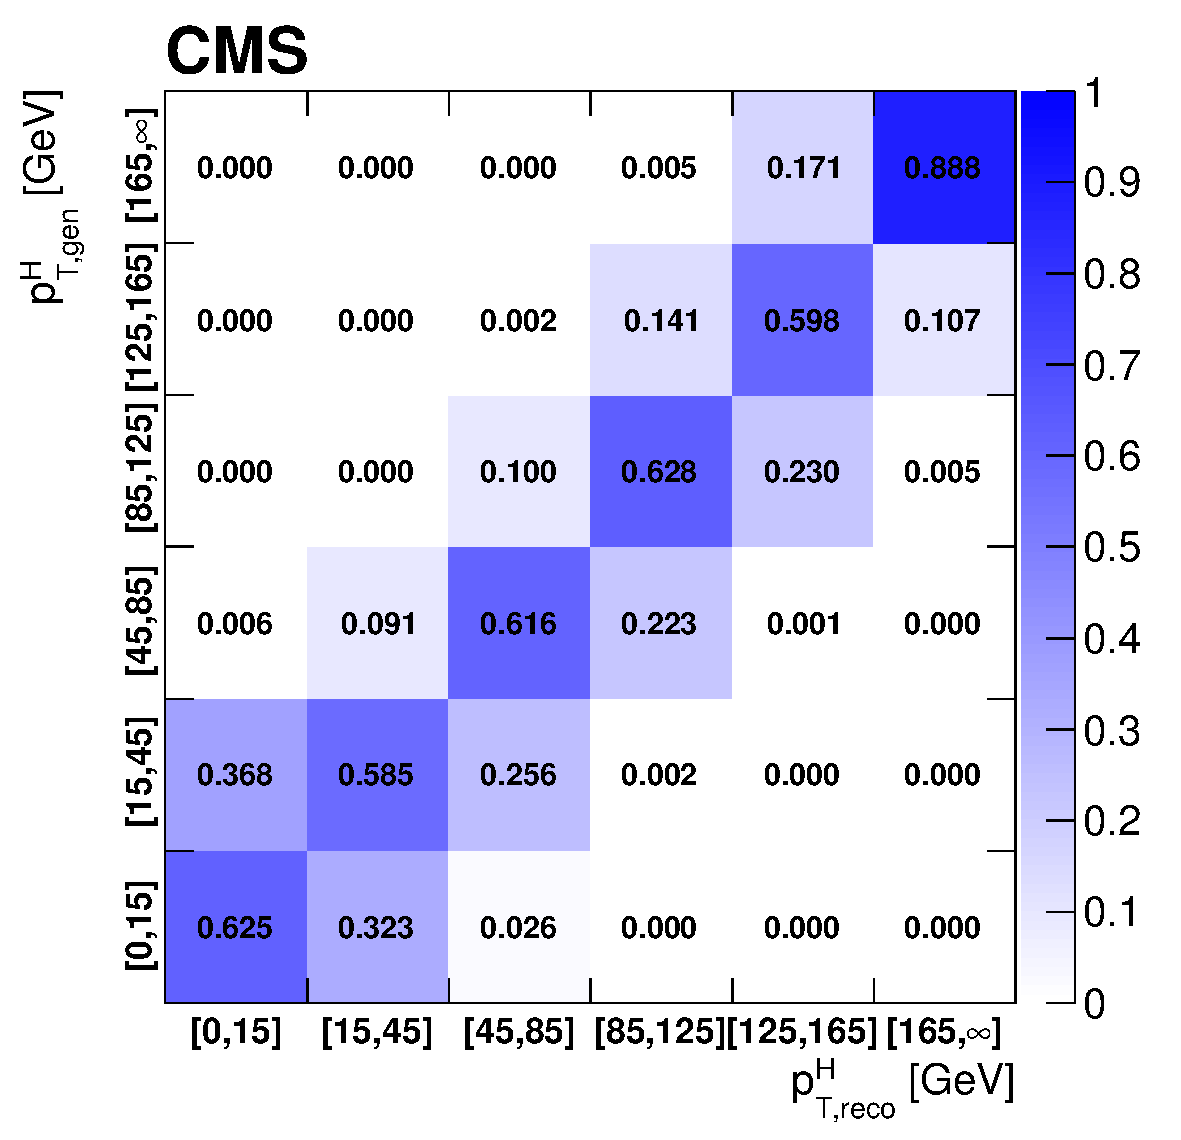
\includegraphics[width=0.45\textwidth]{images/matrix_bycol_paper.pdf}
}
\caption{Response matrix normalized by row (a) and  by column (b) including all signal processes. The matrices are normalized either by row or by column in order to show the purity or stability in diagonal bins.}\label{fig:matrix}
\end{figure}

Several tests are performed in order to validate the unfolding procedure. To estimate the uncertainty in the unfolding procedure due to the
particular model adopted for building the response matrix, two independent ggH samples are used, corresponding to two different generators: \textsc{Powheg V1} and \textsc{JHUGen} generators, both interfaced to \textsc{Pythia 6.4}.
The \textsc{JHUGen} generator sample is used to build the response matrix while the
\textsc{Powheg V1} sample is used to build the \pth spectra at generator and reconstructed level. The reconstructed spectrum obtained using \textsc{Powheg V1} is then unfolded using the response matrix built with \textsc{JHUGen}, and the unfolded spectrum is compared to the \textsc{Powheg V1} spectrum at generator level. The result of this test shows good agreement between the two distributions.

In order to further prove the choice of the regularization parameter, a large number of simulated pseudo-experiments has been generated to verify that the coverage of the unfolded uncertainties obtained with this procedure is as expected.
From each pseudo-experiment the reconstructed \pth spectrum is obtained and then unfolded using the procedure described above, including only the statistical uncertainties. The coverage is calculated for each \pth bin, counting the number of pseudo-experiments for which the statistical uncertainty covers the true value. The results are shown in Table~\ref{tab:coverage} for different values of the regularization parameter: starting from $k_\mathrm{reg}=2$ (stronger regularization) up to $k_\mathrm{reg}=5$ (weaker regularization). The criterion for choosing the best $k_\mathrm{reg}$ value is to increase the regularization as much as possible without introducing a bias, i.e. until a 68\% coverage is fulfilled. This criterion leads to the same result as the prescription described before, strengthening the choice of $k_\mathrm{reg}=3$.

\begin{table}[htb]
\centering
\caption{Coverage interval for each bin and for different values of the regularization parameter, obtained using pseudo-experiments.}\label{tab:coverage}
\begin{tabular}{lcccc}
\toprule
\multirow{2}{*}{\pth bin [GeV]} & \multicolumn{4}{c}{Coverage} \\
 & $k_\mathrm{reg}=2$ & $k_\mathrm{reg}=3$ & $k_\mathrm{reg}=4$ & $k_\mathrm{reg}=5$\\
\midrule
0--15 	      & $0.654\pm0.016$ & $0.704\pm0.015$ & $0.727\pm0.015$ & $0.755\pm0.014$ \\
15--45 	      & $0.701\pm0.015$ & $0.665\pm0.016$ & $0.683\pm0.015$ & $0.733\pm0.015$ \\
45-85 	      & $0.717\pm0.015$ & $0.706\pm0.015$ & $0.709\pm0.015$ & $0.716\pm0.015$ \\
85--125       & $0.634\pm0.016$ & $0.681\pm0.015$ & $0.714\pm0.015$ & $0.739\pm0.015$ \\
125--165      & $0.599\pm0.016$ & $0.650\pm0.016$ & $0.700\pm0.015$ & $0.751\pm0.014$ \\
165--$\infty$ & $0.632\pm0.016$ & $0.674\pm0.015$ & $0.701\pm0.015$ & $0.722\pm0.015$ \\
\bottomrule
\end{tabular}
\end{table}



\subsection{Treatment of systematic uncertainties in the unfolding}\label{sec:uncunf}

An important aspect of this analysis is the treatment of systematic
uncertainties and their propagation through the unfolding procedure.
The sources of uncertainty are divided into three categories, depending
on whether the uncertainty affects only the signal yield (type A), both the signal
yield and the response matrix (type B), or only the response matrix (type C).
These three classes propagate differently through the unfolding procedure.

Type A uncertainties are extracted directly from the fit in the form of a covariance
matrix, which is passed to the unfolding tool as the covariance
matrix of the measured distribution. The nuisance parameters belonging to this category
are the background shape and normalization uncertainties.
To extract the effect of type A uncertainties a dedicated fit is performed fixing to constant all the nuisance parameters in the model but type A ones.
The correlation matrix among the six signal strengths corresponding to the six \pth bins, including all type A uncertainties, is shown in Fig.~\ref{fig:typeA_corr}.
The correlation cor($i$,$j$) of bins $i$ and $j$ is defined as:	
\begin{equation}\label{eq:correlation}
\mathrm{cor}(i,j) = \frac{ \mathrm{cov}(i,j) }{  s_{i}s_{j} } \qquad ,
\end{equation} 

\noindent where $\mathrm{cov}(i,j)$ is the covariance of bins $i$ and $j$, and $s_{i}$, $s_{j}$ are the standard deviations of bins $i$ and $j$,  respectively.

\begin{figure}[htb]
\centering
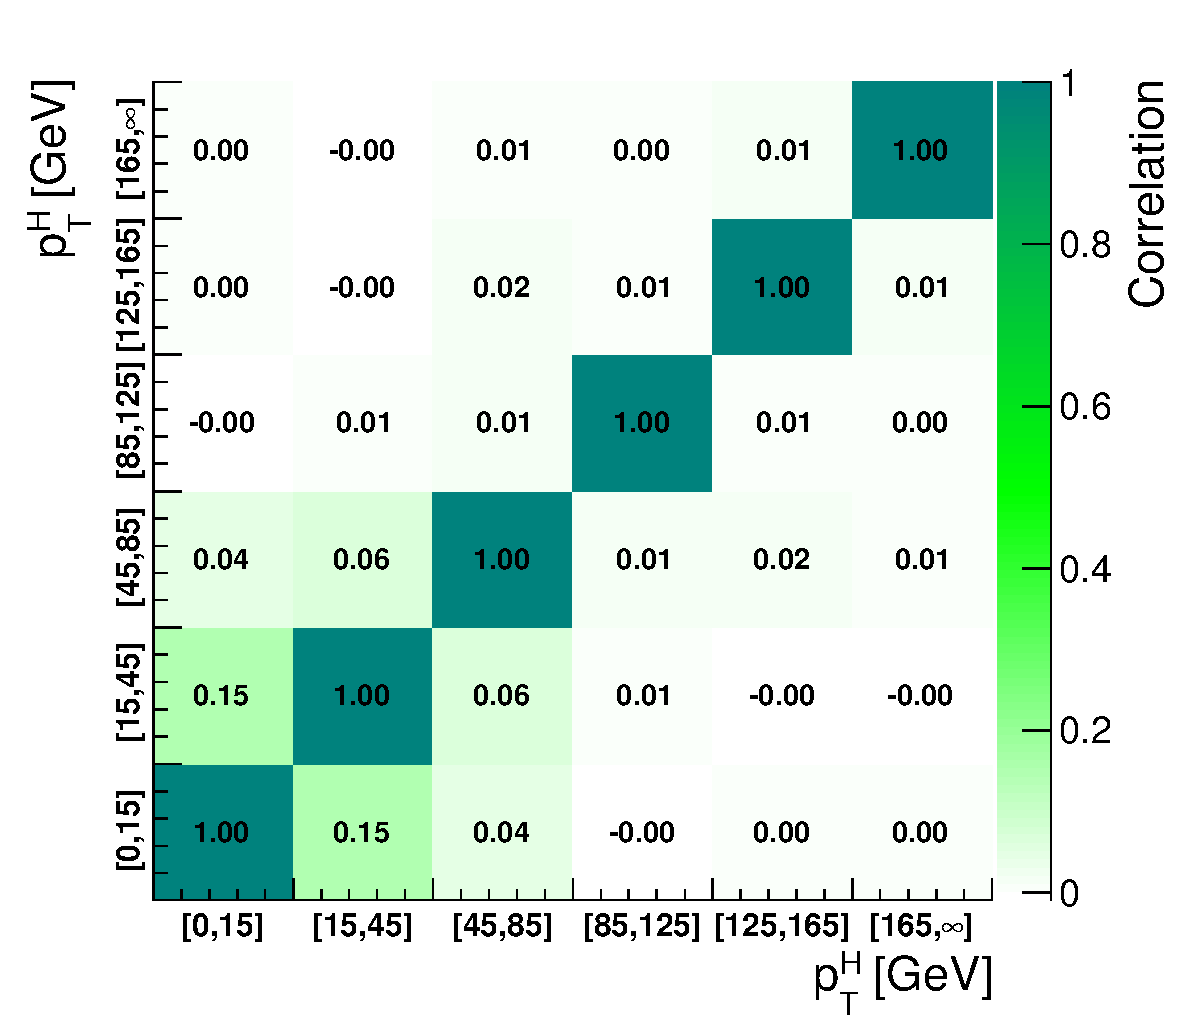
\includegraphics[width=0.6\textwidth]{images/typeACovMatrix.pdf}
\caption{Correlations among the signal strengths corresponding to the six \pth bins including all type A uncertainties.}\label{fig:typeA_corr}
\end{figure}

The nuisance parameters belonging to the Type B class are the ones related to:
\begin{itemize}
\item b veto scale factor: it affects the signal and background templates
by varying the number of events with jets that enter the selection. It also
affects the response matrix because the reconstructed spectrum is harder or softer depending on the number of jets, which in turn depends on the veto;
\item lepton efficiency scale factor: it affects the signal and background
template shape and normalization. It affects the response matrix by varying
the reconstructed spectrum;
\item \MET scale and resolution: the effect is similar to the above;
\item lepton scale and resolution: the effect is similar to the above;
\item jet energy scale: it affects the signal and background template shape
and normalization. It also affects the response matrix because, by varying the
fraction of events with jets, the b veto can reject more or fewer events, thus
making the reconstructed spectrum harder or softer.
\end{itemize}
The effect of each type B uncertainty is evaluated separately,
since each one changes the response matrix in a different way.
In order to evaluate their effect on the signal strengths parameters, two additional fits are
performed, each time fixing  the nuisance parameter value to $\pm 1$  standard
deviation with respect
to its nominal value. The results of the fits are then compared to the results of the full fit obtained by floating  all the nuisance parameters, thus 
determining the relative uncertainty on the signal strengths due to each
nuisance parameter, as shown in Tab.~\ref{table:corr_syst}. 
Using these uncertainties, the measured spectra for each type B
source are built.
The effects are propagated through the unfolding by building the corresponding variations of the response matrix and unfolding the
measured spectra with the appropriate matrix.

Type C uncertainties are related to the underlying assumption on the Higgs boson production mechanism used to extract the fiducial cross sections. These are evaluated using alternative response matrices that are obtained by varying the relative fraction of VBF and ggH components within the experimental uncertainty, as given by the CMS combined measurement~\cite{Khachatryan:2014jba}.
Three different response matrices are built, corresponding to the nominal, scaled up, and scaled down
VBF/ggH ratio. The nominal matrix assumes the SM VBF/ggH ratio, %with $\mu_{\mathrm{ggH}} = \mu_{\mathrm{VBF}} = 1$, 
while up- and down-scaled matrices are constructed by varying the SM signal strengths within the
experimental constraints for VBF and ggH in such a way as to obtain the
maximal variation of the VBF/ggH ratio allowed by the experimental
constraints.
%The VBF/ggH fractions are varied in an anticorrelated way in order to produce the maximum variation of the spectrum shape allowed by the experimental constraints.
These three matrices are used to unfold the reconstructed spectrum with the nominal VBF/ggH fraction, and obtain an uncertainty on the unfolded spectrum.
%It was verified that the variations of the measured spectrum do not affect the shape of the signal templates, \textit{i.e.} \mll~and \mth.

%Type A and B uncertainties are finally combined together after the unfolding
%summing in quadrature positive and negative contributions separately for each bin. Type C uncertainties, also referred to as ``model dependence'', are instead quoted separately.
%The effect of each source of the uncertainty is quoted for each bin of \pth~in Table~\ref{table:values_and_uncertainties}.

\begin{table}[htb]
\caption{Effect of all the Type B uncertainties on the signal strengths of each bin. In the table are reported the signal strength variations corresponding to an up or down scaling of each nuisance parameter. Uncertainties related to \MET and lepton resolution are single-sided, i.e. only an up variation is implemented.}\label{table:corr_syst}
\centering
\footnotesize{
\begin{tabular}{lcccccc}
\toprule
\multirow{2}{*}{Type B uncertainty} & \multicolumn{6}{c}{Effect on signal strength ($+1\sigma/-1\sigma$ [\%])}\\
 		   & [0--15] & [15--45] & [45--85] & [85--125] & [125--165] & [165--$\infty$] \\ 
\midrule
b veto & -10.1/-8.8 & 7.3/12.2 & -6.3/3.1 & -14.4/-4.8 & -5.4/14.5  & -7.9/17.8  \\ 
lepton efficiency & -14.7/-3.9  & 4.5/15.1  & -5.7/2.5  & -13.2/-5.3  & -0.2/7.6  & -0.1/6.8  \\ 
\MET resolution & -12.5/0.0  & 15.4/-0.0  & -12.8/-0.0  & 8.7/0.0  & -20.9/-0.0  & 10.5/0.0  \\
\MET scale & -14.4/-6.8  & -0.0/17.7  & -6.1/-7.1  & 9.6/-20.9  & 2.3/32.4  & 2.5/2.6  \\ 
lepton resolution & -12.5/-0.0  & 11.2/0.0  & -2.4/0.0  & -13.4/-0.0  & 9.9/0.0  & -4.6/-0.0  \\ 
e momentum scale & -2.7/-13.1  & 15.9/9.9  & 10.8/-16.8  & 16.2/-33.1  & 30.9/-14.4  & 12.6/-10.9  \\
$\mu$ momentum scale & -7.0/-10.7  & 11.8/8.9  & 1.1/-8.7  & -0.7/-14.4  & 14.5/-4.6  & 8.0/-1.6  \\ 
jet energy scale & -10.9/-10.1  & 9.0/9.0  & -3.0/-2.9  & -10.3/-8.9  & 0.3/3.4  & 5.2/3.1  \\

\bottomrule
\end{tabular}
}
\end{table}


